\documentclass[../main/main.tex]{subfiles}
\begin{document}
\dominitoc
\faketableofcontents
\setcounter{chapter}{8}
\chapter{Data Release 2 de ZTF}\label{ch:res}

\minitoc
\newpage

\section{Présentation de la DR2 de ZTF}
% \label{sec:xxx}


\begin{table}
  \scriptsize
  \centerfloat
  \setlength\tabcolsep{14pt}
  \renewcommand{\arraystretch}{1.2}
  \begin{threeparttable}

    \caption{Median statistics made from the 431k exposures taken by ZTF during its phase 1.}
    \label{tab:summary_systematics}
    \begin{tabular}{l c c c c c}
      \hline\\[-0.5em]
      \hline\\[-0.5em]
      Filter  & Number of & Seeing & Airmass & Limiting & Cadence\\[0.15em]
              & Exposure & [arcsec] &  & mag [5$\sigma$] &  \\[0.15em]
      \hline\\[-0.5em]
      ztf:g   & 165k & 2.2 & 1.7 & 20.56 & 2.05\\[0.30em]
      ztf:r   & 247k & 2.0 & 1.2 & 20.39 & 1.02\\[0.30em]
      ztf:i   & 19k & 1.8 & 1.1 & 20.03 & 5.03\\[0.30em]
      \hline\\[-0.5em]
      All & 431k & 2.1 & 1.2 & 20.42 & 2.96\\[0.30em]
    \end{tabular}
    \begin{tablenotes}[flushleft]
    \item \textbf{Note.}Only images with no bad-quality flags are considered. 
      Cadence is per field and per filter, so cadence “All” is the
      median cadence per field and per filter.
    \end{tablenotes}
  \end{threeparttable}
\end{table}
    

\begin{figure}[ht]
  \centering
  \makebox[\textwidth][c]{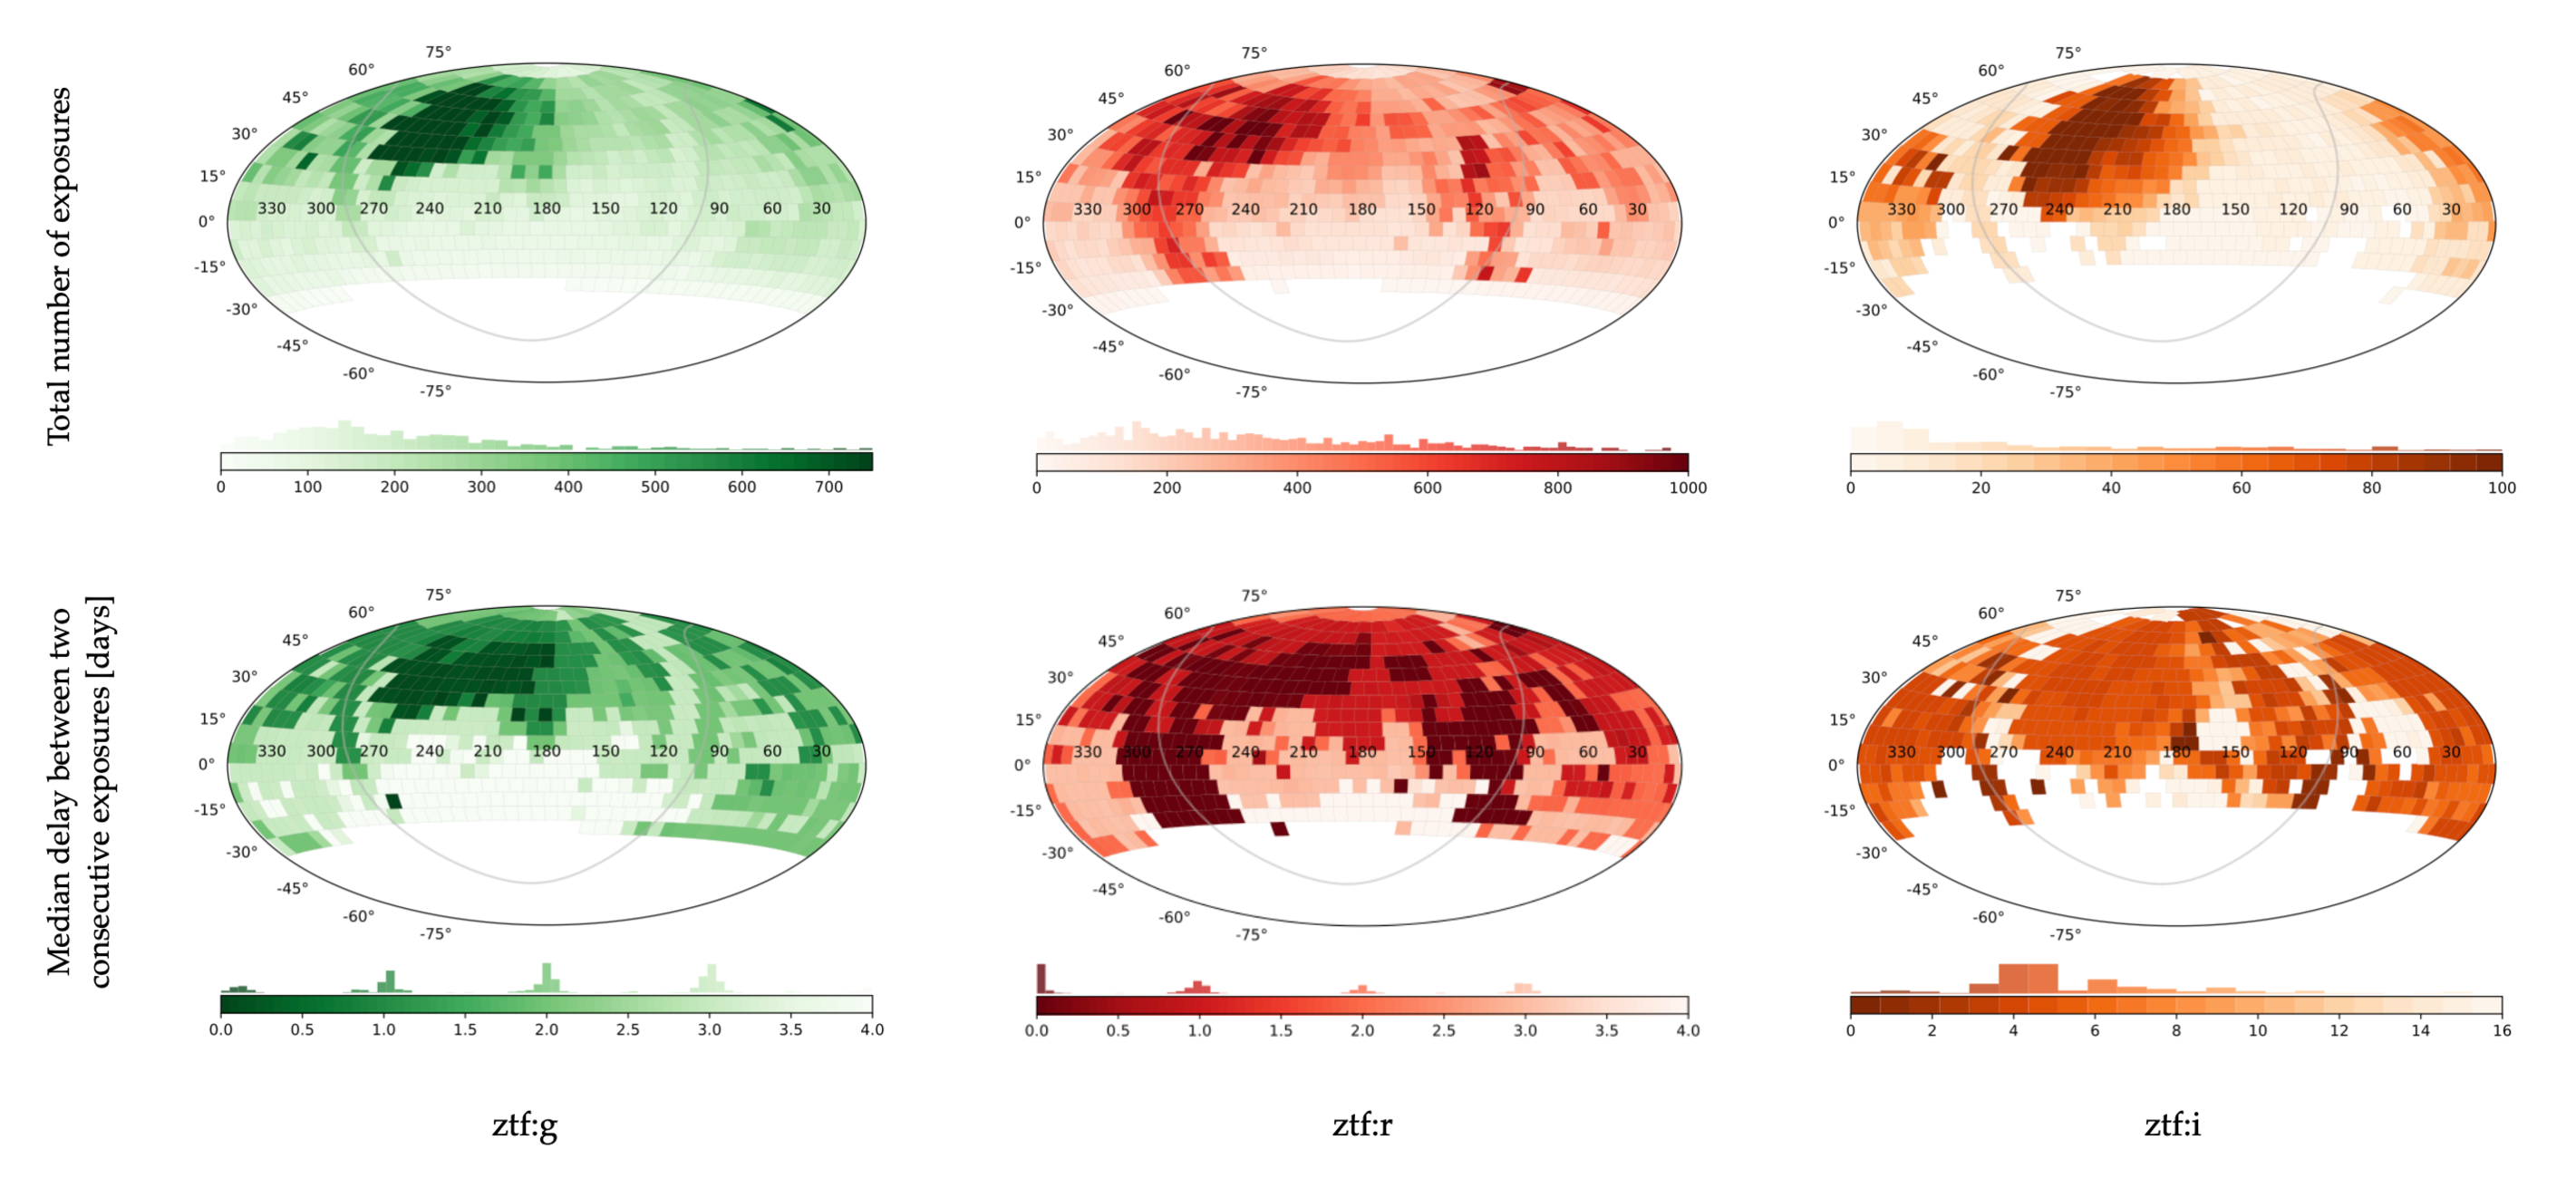
\includegraphics[width=1.15\textwidth]{../figures/09_dr2/ztf_skycoverage_and_cadence_landscape_lowq.pdf}}%
  \caption[]{}
  \label{fig:skycoverage}
\end{figure}


\section{Statistiques sur les supernovae de type Ia}
%\label{sec:xxx}

\subsection{Classification spectrale}
%\label{ssec:xxx}

\begin{figure}[ht]
  \centering
  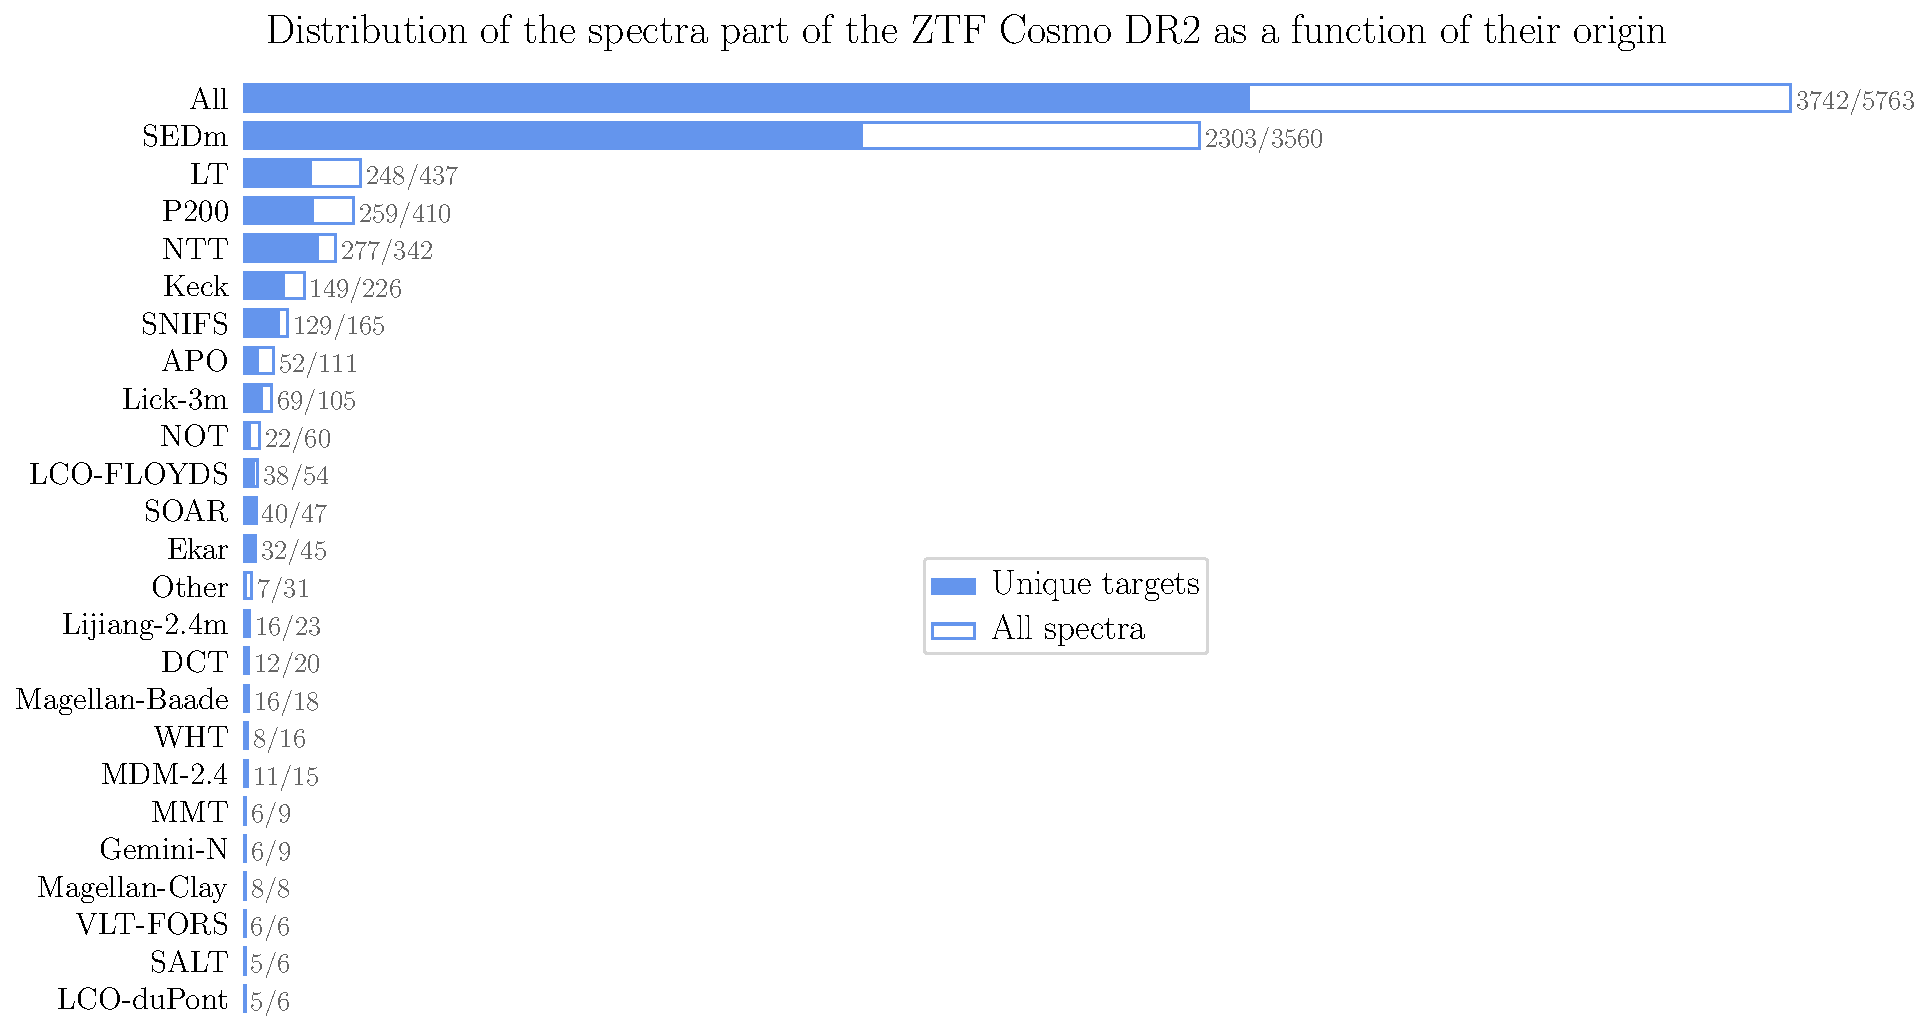
\includegraphics[width=1\textwidth]{../figures/09_dr2/spec_instorigin_dr2.pdf}
  \caption[]{}
  \label{fig:specorigindr2}
\end{figure}

\begin{figure}[ht]
  \centering
  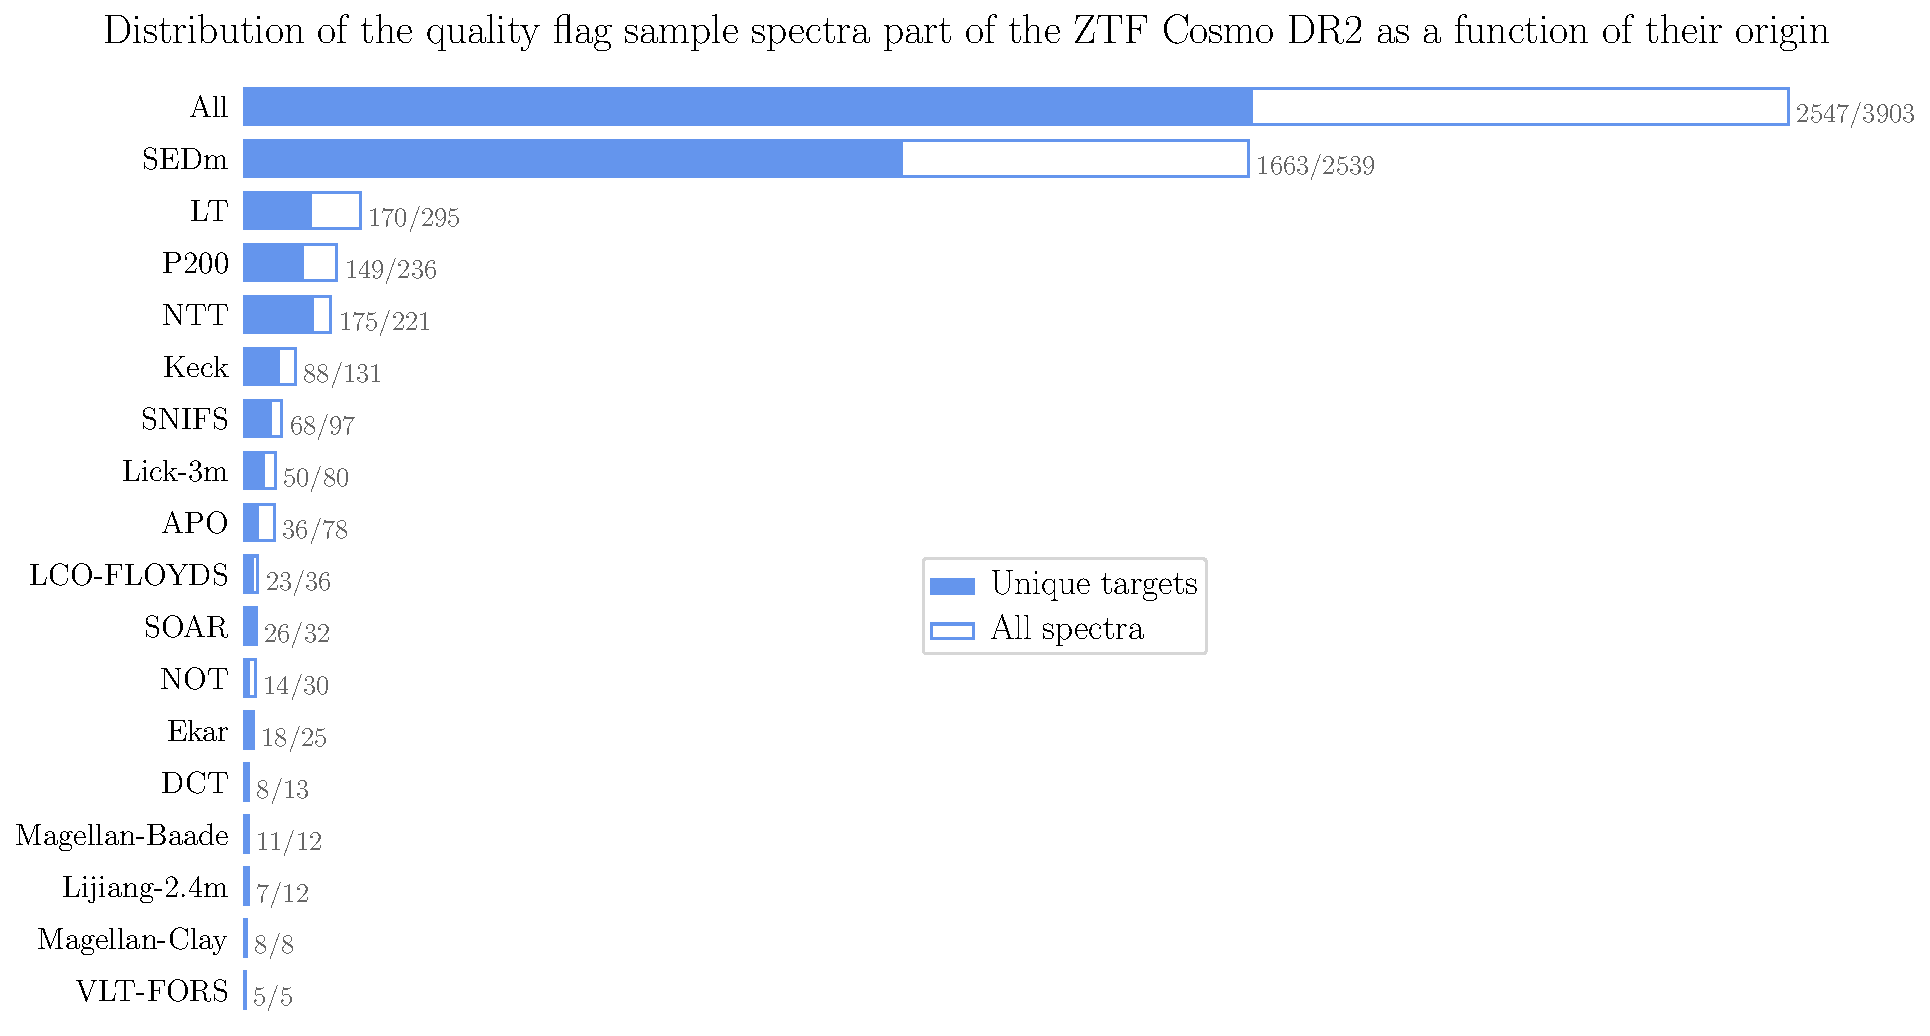
\includegraphics[width=1\textwidth]{../figures/09_dr2/spec_instorigin_golden_dr2.pdf}
  \caption[]{}
  \label{fig:specorigingoldendr2}
\end{figure}

\subsection{Photométrie}
% \label{ssec:xxx}


\begin{figure}[ht]
  \centering
  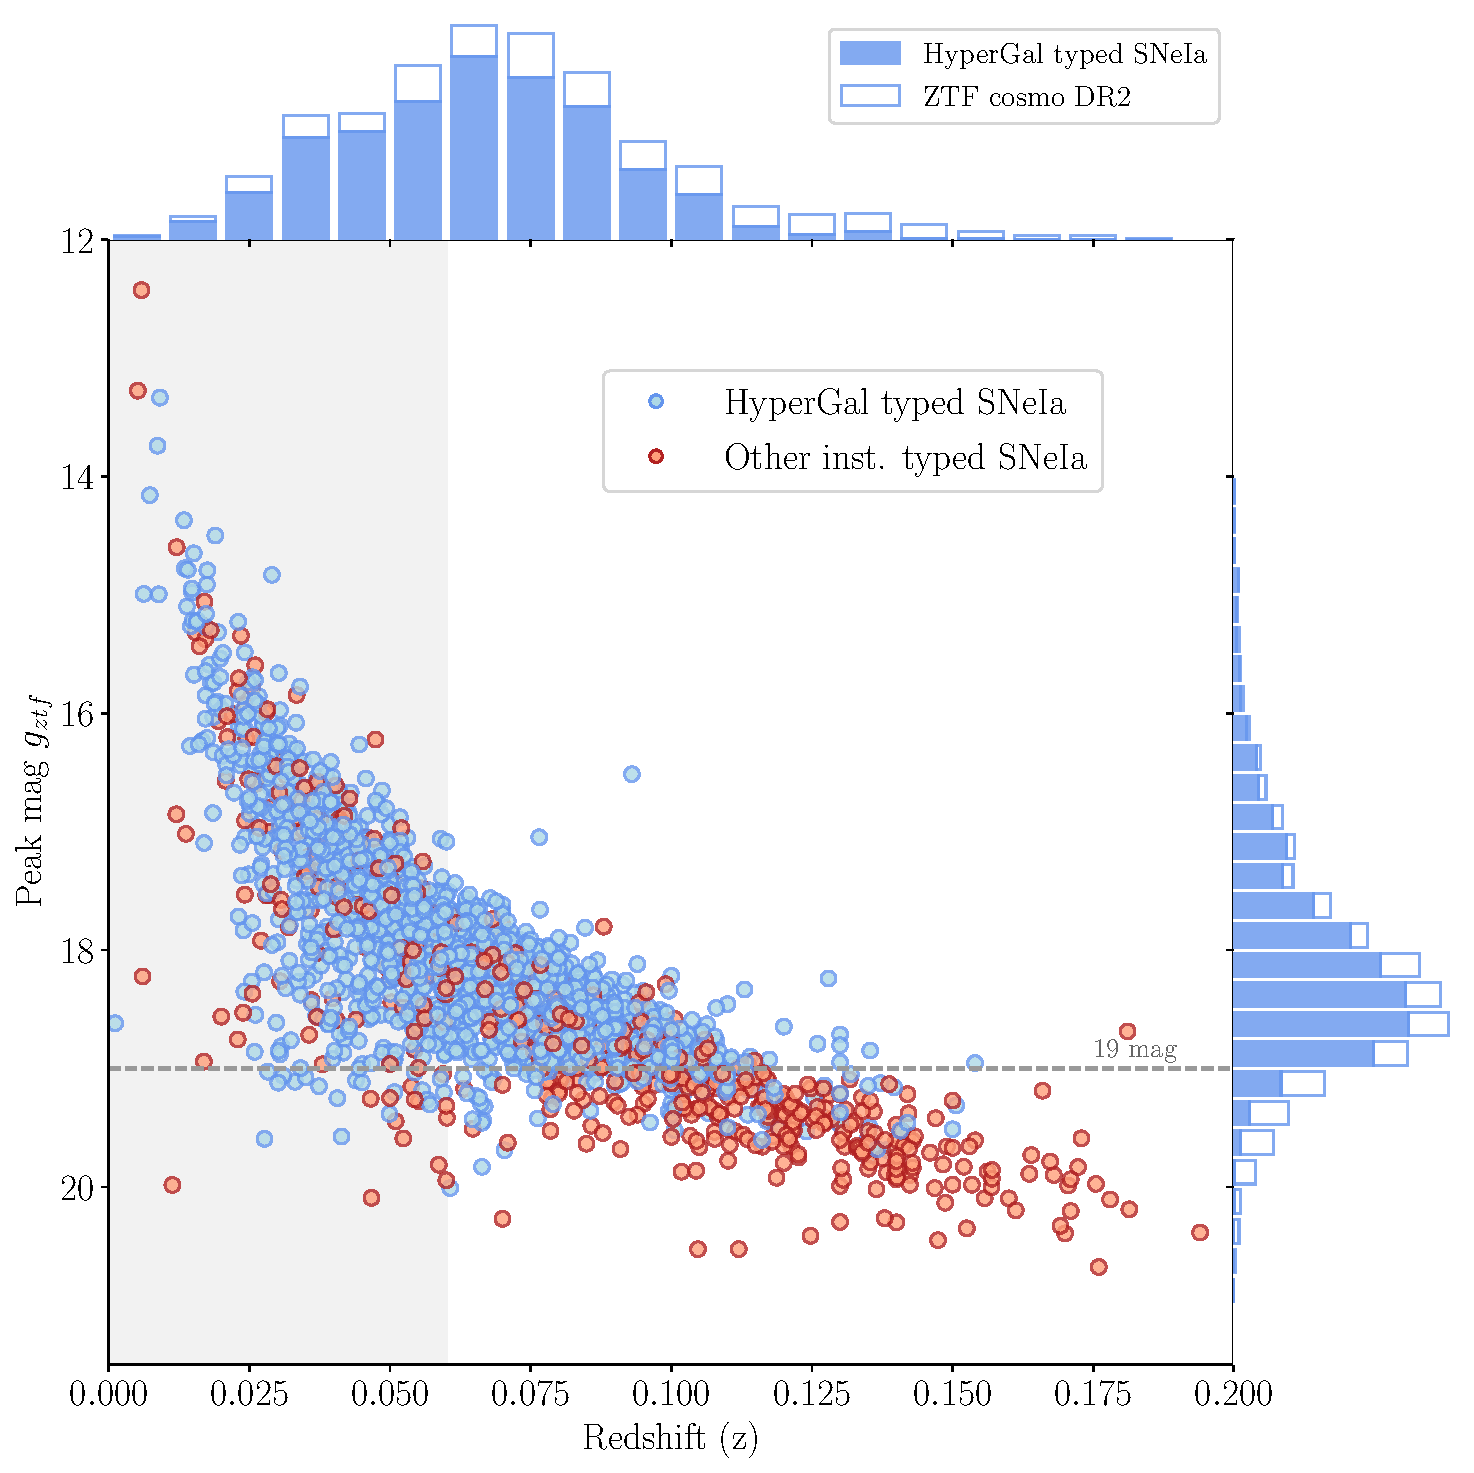
\includegraphics[width=1\textwidth]{../figures/09_dr2/peakvsredshift_dr2.pdf}
  \caption[]{}
  \label{fig:peakmagztfg}
\end{figure}

\subsection{Courbes de lumière}


\begin{figure}[ht]
  \centering
  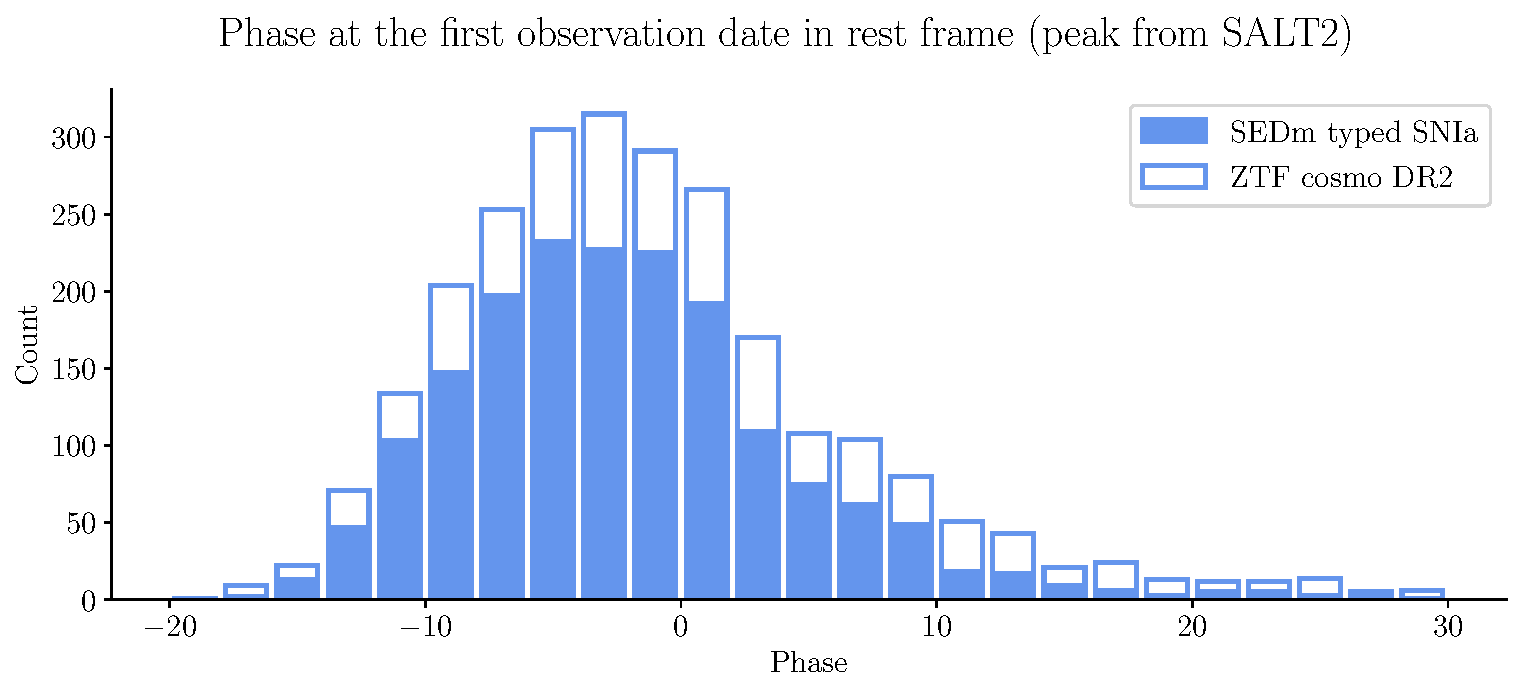
\includegraphics[width=1\textwidth]{../figures/09_dr2/phaseIadr2.pdf}
  \caption[]{}
  \label{fig:phaseIa}
\end{figure}


L'utilisation de l'échantillon de SNeIa pour dériver les paramètres
cosmologiques nécessite de considérer d'éventuels biais de sélection. En
effet, une SNIa avec un paramètre de couleur élevé (donc plus rouge) ou
un déclin rapide de luminosité (bas stretch) peuvent ne plus être détectées
par ZTF et sa profondeur en magnitude limite. La
Figure~\ref{fig:ztfdr2salt} met bien en évidence cet effet de sélection,
où la corrélation entre les paramètres de la courbe de lumière et le
redshift est clairement visible. C'est pourquoi un sous-échantillon à
volume limité ($z<0.06$) est considéré, comme indiqué par \textbf{Amenouche et al (in prep)} .

\begin{figure}[ht]
  \centering
  \makebox[\textwidth][c]{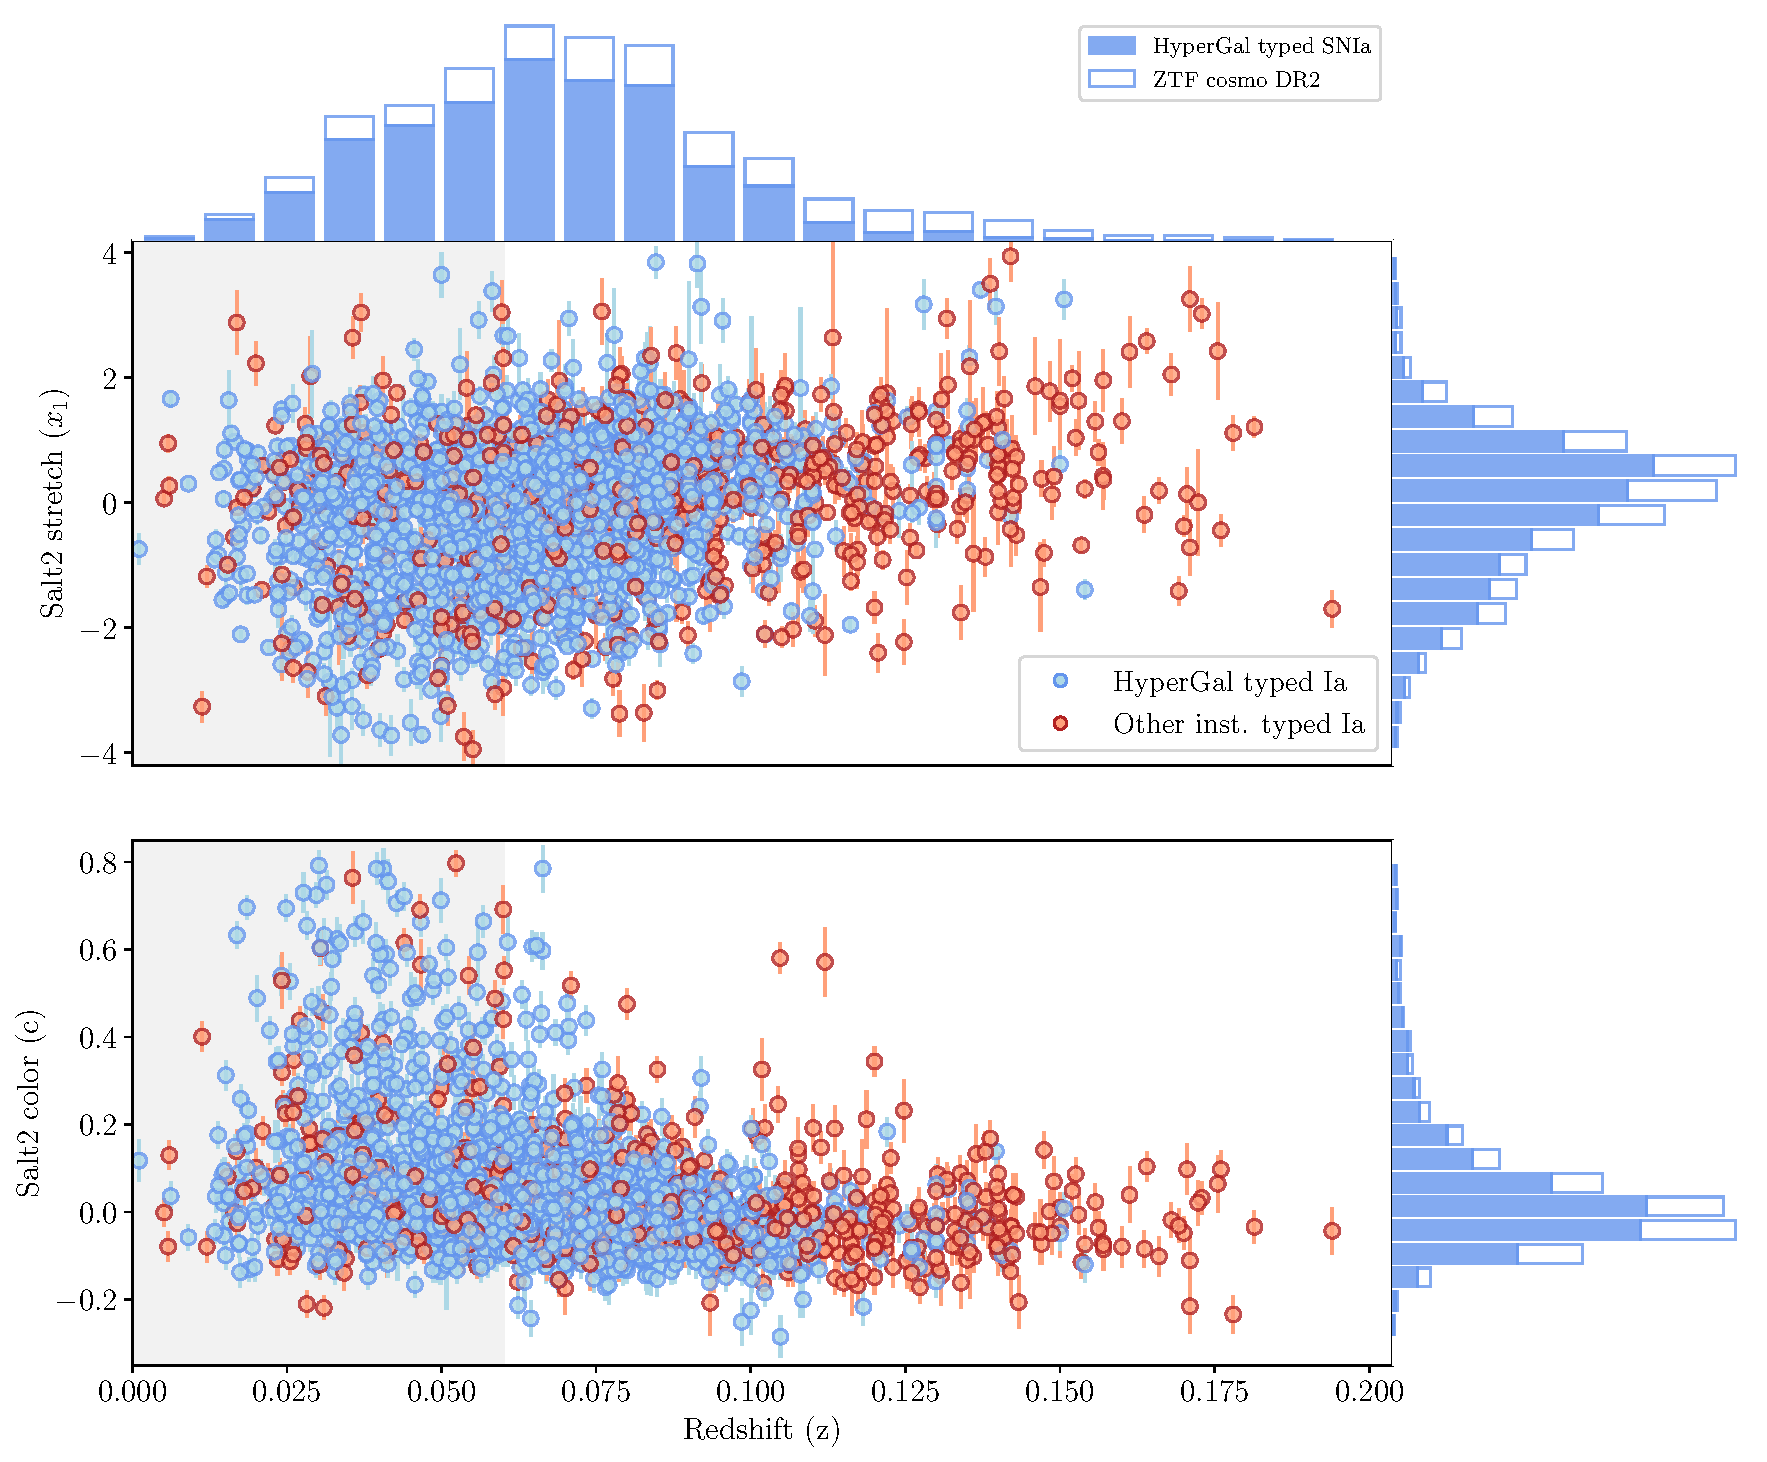
\includegraphics[width=1.1\textwidth]{../figures/09_dr2/stretch_color_redshift_dr2.pdf}}%
  \caption[Paramètres SALT2 de stretch et couleur pour la DR2 de
  ZTF]{Paramètres SALT2 de stretch (\textit{en bas}) et couleur
    (\textit{en haut}) pour la DR2 de ZTF (\textbf{Rigault et al DR2 (in prep)}). Ici seules les Supernovae de
    l'échantillon doré son considérées. La bande grise indique le
    volume limite à $z<0.06$. Les histogrammes sur la droites
    représentent l'échantillon entier (en bleu) et volume limité (en gris).}
  \label{fig:ztfdr2salt}
\end{figure}

Le volume limité étant défini, il est à présent possible d'étudier les
paramètres de distributions des courbes de lumières, ainsi que leurs
corrélations. La première raison de cette analyse est la nécessité
d'estimer la fonction de sélection sous-jacente pour éviter d'induire
des biais dans la dérivation des
paramètres cosmologiques \citep{Scolnicbias2016}. La seconde raison est
que cela permet d'étudier la nature de la population (jeune/vieille) des
SNIa, et de mettre en évidence des potentiels évolution en redshift
\citep{NoraNicolas21}. Les corrélations stretch/couleur sont montrées
dans la Figure~\ref{fig:ztfdr2saltcorr}, où la caractéristique bi-modale
de la distribution en stretch est clairement visible. Le mode à bas
stretch compte pour $\approx25\%$ de la distribution, comme prédit par \citet{NoraNicolas21}.

\begin{figure}[ht]
  \centering
  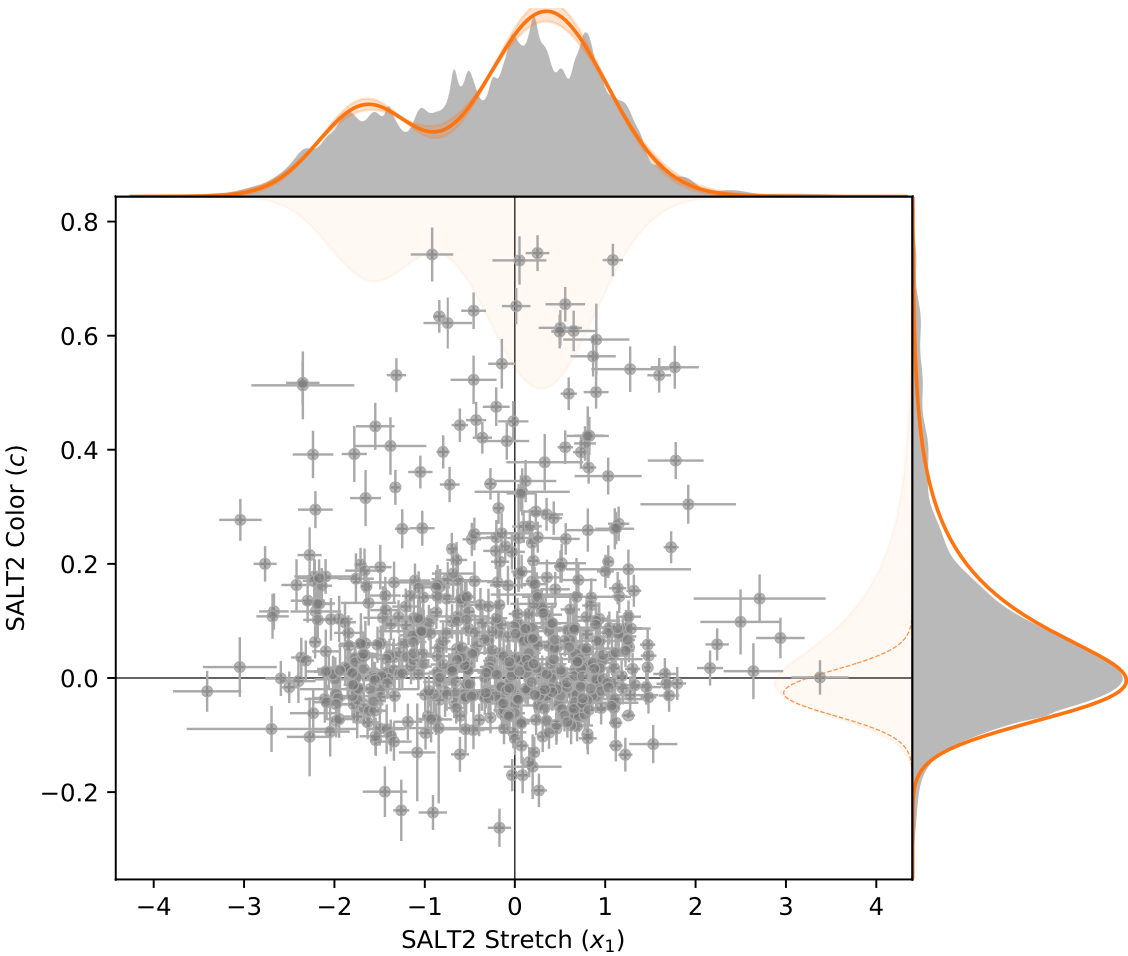
\includegraphics[width=1\textwidth]{../figures/02_ztf/ztfdr2stretchcolorcorrelation.png}
  \caption[Correlation entre les paramètres SALT2 de stretch et couleur
  (ZTF-DR2)]{ Correlation entre les paramètres SALT2 de stretch et
    couleur pour la DR2 de ZTF (\textbf{Rigault et al DR2 (in prep)}). Ici seules les Supernovae du
    volume limité à $z<0.06$ sont considérées. Les distributions en
    orange correspondent aux prédictions du model de double population
    de SNeIa de \citet{NoraNicolas21}.}
  \label{fig:ztfdr2saltcorr}
\end{figure}



\subsection{Des SNeIa à la cosmologie: $H_{0}$, $w$ et $f\sigma_{8}$} \label{sec:sniaztfcosmo}

À ce rythme, ZTF aura observé et classifié près de $5000$ SNeIa de
qualité cosmologique d'ici la
fin de la phase 2, mi-2024.

\bibliographystyle{../main/aa_url2}
\bibliography{99_references}
\end{document}

%%% Local Variables:
%%% mode: latex
%%% TeX-master: t
%%% End:
